
Deux signaux sonores S1 et S2 échantillonnés à 44.1 kHz


S1 comporter que deux composantes audibles sous la forme de deux sinusoïdes de fréquences 1000 et 3000 Hz.
\\
S1=$2*sin(2*pi*1000*t) .+ 5*sin(2*pi*3000*t)$


\begin{figure}[H]
\centering
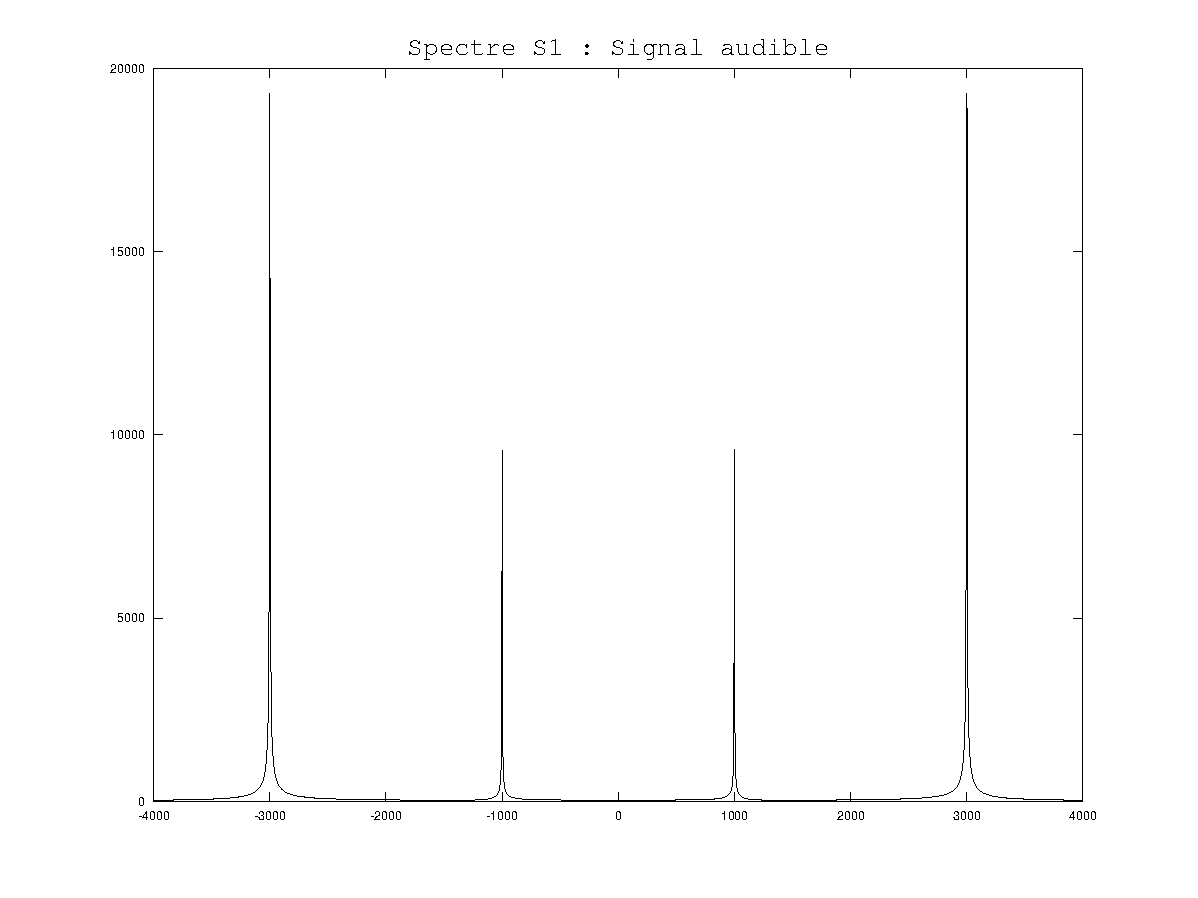
\includegraphics[width=9cm]{resEx7/s1_audible.pdf}
\caption{Spectre de S1}
\end{figure}

Le spectre de fréquence permet de voir les 2 composantes à 1kHz et à 3kHz.
\\\\\\


S2 comporte un signal inaudible à 43.5 kHz: S2=$5*sin(2*pi*43100*t)$

\begin{figure}[H]
\centering
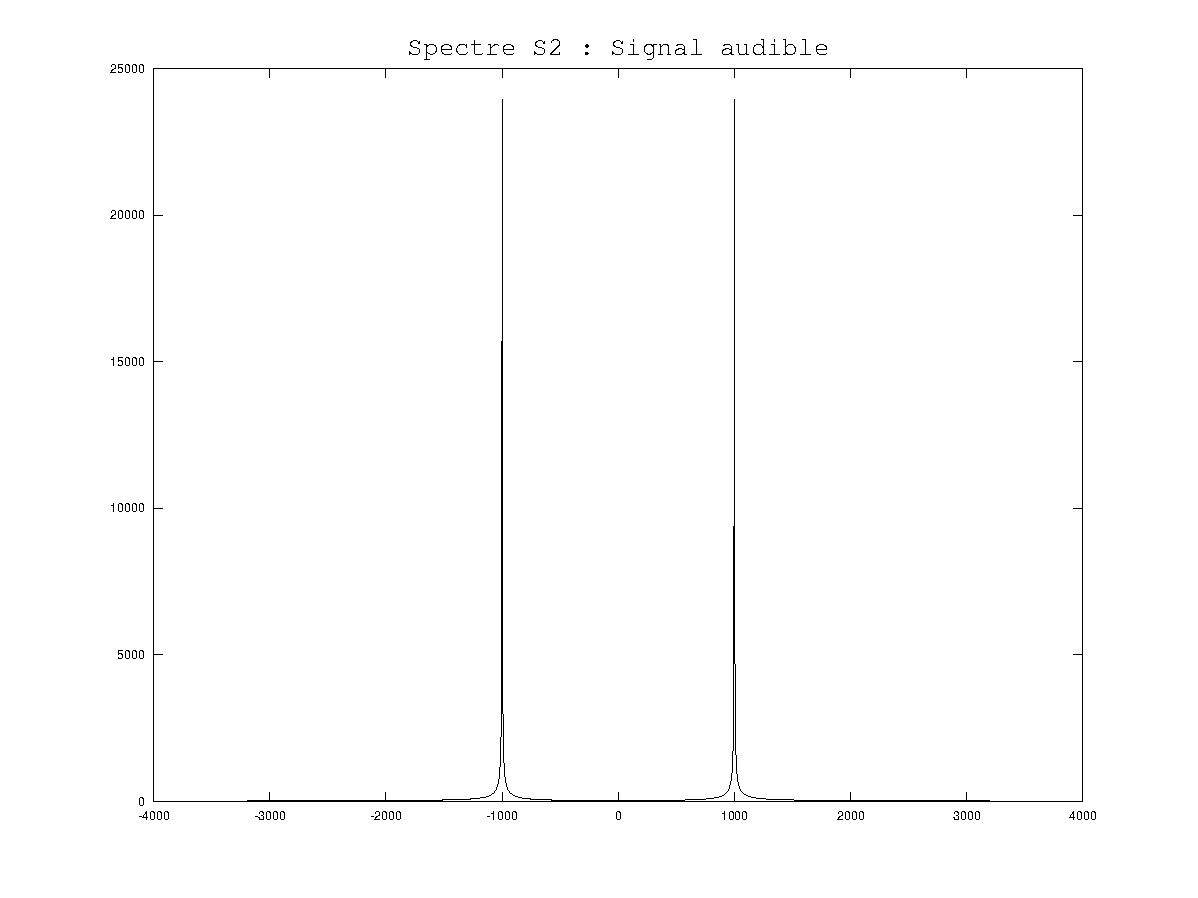
\includegraphics[width=9cm]{resEx7/s2_inaudible.pdf}
\caption{Spectre de S2}
\end{figure}

La fréquence du signal inaudible ne respecte pas la condition de Shannon.

En effet, si on veut échantillonner sans perdre d'information un signal à spectre limité, il faut échantillonner ce signal à une fréquence au moins égale au double de la plus haute fréquence qu'il contient.


